\section{Technical Overview}

To put our work into context, we give a brief overview of \aal~\cite{SP:TaiMorMaf21} recast as a synchronization puzzle (a notion first introduced in~\cite{NDSS:HABSG17}), and discuss how it can be used as a coin mixing protocol. We then outline the vulnerabilities in \aal and discuss how to fix them using the tools that we develop in this work.

\begin{figure}[tbh]
    \centering
    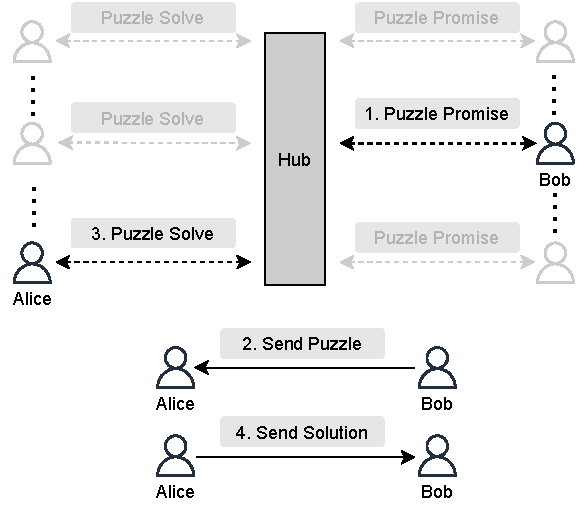
\includegraphics{bcs/figs/bcs.pdf}
    \caption{Protocol flow of the \syncpuzzle, the underlying cryptographic mechanism of Tumblebit and \aal. Our approach in Blind Conditional Signatures follows a similar execution. Dotted double-edged arrows indicate 2-party protocols. Solid arrows indicate secure point-to-point communication.}
    \label{fig:sync_tool}
\end{figure}

\paragraph{Synchronization Puzzles} A \syncpuzzle protocol is a protocol between three parties: Alice, Bob, and Hub (refer to~\Cref{fig:sync_tool} for a depiction). The \syncpuzzle begins with Hub and Bob executing a \emph{puzzle promise} protocol (step 1) with respect to some message, $m_\hb$ such that Bob receives a puzzle $\tau$ that contains a signature $s$ (at this point still hidden) on $m_\hb$. Bob wishes to solve the puzzle and obtain the embedded signature. To do this, he sends the puzzle $\tau$ privately to Alice (step 2), who executes a \emph{puzzle solve} protocol (step 3) with Hub with respect to some message $m_\ah$ such that, at the end of the protocol, Alice obtains the signatu $s$, whereas Hub obtains a signature $s'$ on $m_\ah$.
Alice then sends the signature $s$ privately to Bob (step 4). Such a protocol must satisfy the following properties.

\smallskip\noindent\underline{Blindness:} The puzzle solve protocol does not leak any information to Hub about $\tau$, and Hub \emph{blindly} helps solve the puzzle. This ensures that Hub cannot link puzzles across interactions.

\smallskip\noindent\underline{Unlockability:} If step 3 is successfully completed, then the secret $s$ must be a valid secret for  Bob's puzzle $\tau$. This guarantees that Hub cannot learn a signature on $m_\ah$, without at the same time revealing a signature on $m_\hb$.

\smallskip\noindent\underline{Unforgeability:} Bob cannot output a valid signature on $m_\hb$ before Alice interacts with the Hub.


{\paragraph{Towards a Coin Mixing Service}
As shown in~\cite{NDSS:HABSG17,SP:TaiMorMaf21},  the \syncpuzzle is the cryptographic core of a coin mixing service. First, Alice and Bob define the messages $$m_\ah: (A \xrightarrow{~v~} H) \text{ and }m_\hb: (H \xrightarrow{~v~} B)$$ where $(U_i \xrightarrow{~v~} U_j)$ denotes a cryptocurrency payment (e.g., on-chain transaction or a payment over payment channels) that transfers $v$ coins from $U_i$ to $U_j$. Second, Alice and Bob run the \syncpuzzle protocol with Hub to synchronize the two aforementioned transfers. Here, 
the signatures $s$ and $s'$ are the ones required to validate the transactions defined by $m_\ah$ and $m_\hb$. The anonymity of mixing follows from the fact that multiple pairs of users are executing the \syncpuzzle simultaneously with Hub, and Hub cannot link its interaction on the left to the corresponding interaction on the right.}
Throughout the rest of this work, we mainly focus on the \syncpuzzle as a cryptographic primitive. The application of a coin mixing protocol follows as prescribed in prior works~\cite{NDSS:HABSG17,SP:TaiMorMaf21}.


\paragraph{The \aal System} In \aal, the \emph{blindness} property is achieved by making use of a re-randomizable linearly homomorphic (CPA-secure) encryption. The puzzle $\tau$ contains a ciphertext $c \gets \enc(\ek_H,\allowbreak s)$ encrypting the signature $s$ under the encryption key $\ek_H$ of Hub. During the puzzle solve step, Alice first re-randomizes the ciphertext (and the underlying plaintext)
$$
c \xrightarrow{~r~} c' = \enc(\ek_H, s + r)
$$
with a random scalar $r$. Hub then decrypts $c'$ to obtain $s+r$, which in turn reveals a signature $s'$ on $m_\ah$.\footnote{This is achieved via the notion of \emph{adaptor signatures}, but for the sake of this overview we ignore the exact details of this aspect.} Alice can then strip off the re-randomization factor $r$ and send $s$ to Bob later in step 4. In the analysis, it is argued that the CPA-security of the encryption scheme ensures unforgeability, whereas the re-randomization process guarantees blindness. Unfortunately, we show in this work that this claim is flawed.

\paragraph{Counterexamples} We observe that the encryption scheme is only CPA-secure, and the Hub is offering a decryption oracle in disguise. In these settings, the right notion of security is the stronger CCA-security, which accounts exactly for this scenario. However, CCA-security is at odds with blindness, since we require the scheme to be (i) linearly homomorphic and (ii) publicly re-randomizable.\footnote{It is well known that no encryption scheme that satisfies either of these properties can be CCA-secure.} We then substantiate this concern by showing two counterexamples. Specifically, we show that there exist two encryption schemes that satisfy the prerequisites spelled out by \aal, but enable two concrete attacks against the protocol. Depending on the scheme, we can launch one of the following attacks:
\begin{itemize}
    \item A key recovery attack that completely recovers the long-term secret key of the hub, i.e., the decryption key $\dk_H$.
    \item A one-more signature attack that allows one to obtain $n+1$ signatures on transactions from Hub to Bob, while only revealing $n$ signatures on transactions from Alice to Hub. Effectively, this allows one to steal coins from the hub.
\end{itemize}
We stress that both these schemes are specifically crafted to make the protocol fail: their purpose is to highlight a gap in the security model of \aal. As such, they do not imply that \aal as implemented is insecure, although we cannot prove it secure either. For a detailed description of the attacks, we refer the reader to~\Cref{sec:attack1}.

\paragraph{Can We Fix This?} In light of our attacks, the natural question is whether we can establish formally rigorous security guarantees for the (appropriately patched) \aal system. While it seems unlikely that \aal can achieve UC-security (more discussion on this later), we investigate whether it satisfies some weaker, but still meaningful, notion of security. Our main observation here is that a weak notion of CCA-security for encryption schemes suffices to provide formal guarantees for \aal. This notion, which we refer to as \emph{one-more CCA-security}, (roughly) states that it is hard to recover the plaintexts of $n$ ciphertexts while querying a decryption oracle at most $n-1$ times. Importantly, this notion is, in principle, not in conflict with the homomorphism/re-randomization requirements, contrary to standard CCA-security.

Towards establishing a formal analysis of \aal, we introduce the notion of blind conditional signatures (BCS) as the cryptographic cornerstone of a \syncpuzzle. We propose game-based definitions (\Cref{sec:bcs-defs}) similar in spirit to the well-established security definitions of regular blind signatures~\cite{C:Chaum82,JC:SchUnr17}. We then prove that \aalplus, our appropriately modified version of \aal, satisfies these definitions (\Cref{sec:modified-a2l}). Our analysis comes with an important caveat: we analyze the security of our scheme in the \emph{linear-only encryption model}. This is a model introduced by Groth~\cite{TCC:Groth04} that only models adversaries that are restricted to perform ``legal'' operations on ciphertexts, similarly to the generic/algebraic group model. While this is far from a complete analysis, it increases our confidence in the security of the system.\footnote{We resort to the LOE model because of the seemingly inherent conflict between linear homomorphism and CCA-like security, both of which are needed for our application (in our setting, the adversary has access to something akin to a decryption oracle). Indeed, even proving that ElGamal encryption is CCA1-secure in the standard model is a long-standing open problem, and we believe that the \aal approach would inherently hit this barrier without some additional assumption.}

\paragraph{UC-Security} The next question that we set out to answer is whether we can construct a \syncpuzzle that satisfies the strong notion of UC-security. We do not know how to prove that \aal (or \aalplus) is secure under composition, which is why we prove \aalplus secure only in the game-based setting. The technical difficulty in proving UC-security is that blindness is unconditional, and we lack a ``trapdoor mechanism'' that allows the simulator to link adversarial sessions during simulation in the security analysis; the proof of UC-security in \cite{SP:TaiMorMaf21} is flawed due to this same reason. Thus, in~\Cref{sec:our_protocol} we develop a different protocol (called \aaluc) that we can prove UC-secure in the standard model. The scheme relies on standard general-purpose cryptographic tools, such as 2PC, and incurs a significant increase in computation costs. We stress that we view this scheme as a proof-of-concept, and leave further improvements for practical efficiency as an open problem.  We hope that the scheme will shed some light on the barriers that need to be overcome in order to construct a practically efficient UC-secure \syncpuzzle.